\chapter{Learning the basics}
Hazelcast is a clustering and highly scalable data distribution platform for Java. It is written in Java, so there is no native part and it can be used in an Language running on top of the JVM.

\begin{enumerate}
  \item distributed collections like BlockingQueue, Map, Set etc.
  \item distributed primitives like locks, semaphore, countdownlatches etc.
  \item distributed execution of tasks, so tasks can be submitted on one JVM and executed 
        on another.
  \item Scaling to hundreds of servers; just add more nodes to add additional capacity to your clustered system.
  \item Providing high availability; so if one node in the cluster fails anther node will take over.
\end{enumerate}

\section{Installing Hazelcast}
First you need to make sure that Java 5 or higher is installed on your machine. If not installed, it can be downloaded from the Oracle site: http://java.com/en/download/index.jsp. After you ensured that Java is installed.

Hazelcast can be downloaded from http://www.hazelcast.com/downloads.jsp. There are 2 versions:
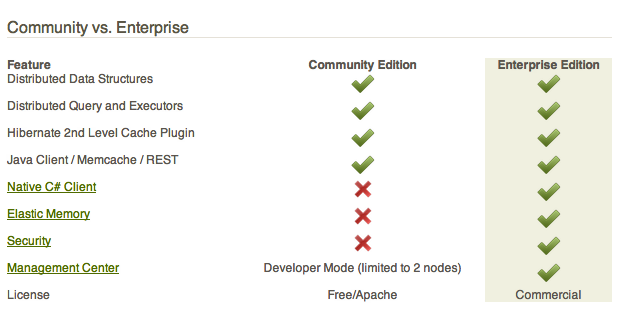
\includegraphics[scale=0.60]{hazelcast-editions.png}
For the purpose of this book we'll use the community edition. If your project relies on Maven, there is no need to install Hazelcast. Setting the dependencies is enough, see next chapter.

If your project is not relying on Maven, then make sure that the Hazelcast jar is added to the classpath, there is no need to install Hazelcast.

\section{Hazelcast and Maven}
Hazelcast is very easy to include in your Maven project without needing to install Hazelcast at all. Hazelcast can be found in the standard Maven repositories, so no need to added additional repositories to your Maven project. To include Hazelcast in your project, just add the following to your pom.xml:
\begin{lstlisting}[language=xml]
<dependencies>	
   ...
   <dependency>
      <groupId>com.hazelcast</groupId>
      <artifactId>hazelcast</artifactId>
      <version>2.3.1</version>
   </dependency>
</dependencies>
\end{lstlisting}
That is it. Make sure that you check the Hazelcast website to make use of the most recent version. 

After this dependency is added, Maven will automatically downloaded the dependencies needed.  The lack of needing to install Hazelcast is something I really like because it saves up quite a lot of time, so we can spend that time doing more useful things.

\section{Configuring Hazelcast}
Hazelcast can be configured in different ways:
\begin{enumerate}
\item xml-configuration file
\item programmatic 
\item Spring
\end{enumerate}
In this book we'll use the xml configuration file. When you are running a maven project; just add a resources directory under your src/main/ and create a file 'hazelcast.xml'. The following xml shows an empty configuration:
\begin{lstlisting}[language=xml]
<hazelcast xsi:schemaLocation="http://www.hazelcast.com/schema/config
                               http://www.hazelcast.com/schema/config/hazelcast-config-2.5.xsd"
           xmlns="http://www.hazelcast.com/schema/config"
           xmlns:xsi="http://www.w3.org/2001/XMLSchema-instance">
</hazelcast>
\end{lstlisting}
This example also imports and XML schema (XSD) for validation and if you are using an IDE, you probably get code completion. To reduce the size of the examples, the XSD import is left out.

In our examples we rely on multicast being enabled for member discovery. So if an XML configuration file is going to be used, it needs to contain the following:
\begin{lstlisting}[language=xml]
<hazelcast>
    <network>
       <join><multicast enabled="true"/></join>
   </network>
</hazelcast>
\end{lstlisting}
For more information check [chapter Cluster Configuration: Multicast]
[todo: verify.. an empty network configuration doesn't automatically multicast?]

In this book, and probably also in practice, will be using the following approach to load a HazelcastInstance:
\begin{lstlisting}[language=java]
public class Main {
    public static void main(String[] args){
        HazelcastInstance hzInstance = Hazelcast.newHazelcastInstance();
        ...
    }
}
\end{lstlisting}
With this approach Hazelcast will use the following mechanism to configure itself:
\begin{enumerate}
\item checks if the 'hazelcast.config' system property is set. This is useful if you want to make use of an external configuration file that is not embedded in the project jar(s). This config option can be set by adding the following to the java command: '-Dhazelcast.config=<path to the hazelcast.xml>' 
\item check if there is a 'hazelcast.xml' available on the classpath. 
\item loads the default hazelcast configuration based on the 'hazelcast-default.xml' that is part of the Hazelcast jar
\end{enumerate}

Another option to load a HazelcastInstance is to make use of programmatic configuration, e.g: 
\begin{lstlisting}[language=java]
public class Main {
    public static void main(String[] args){
        Config config = new Config();
                
        NetworkConfig newWorkConfig = config.getNetworkConfig();
        Join join = newWorkConfig.getJoin();
        join.getMulticastConfig().setEnabled(false);
                
        MapConfig mapConfig = new MapConfig();
        mapConfig.setName("testMap");
        mapConfig.setBackupCount(2);
        mapConfig.getMaxSizeConfig().setSize(10000);
        mapConfig.setTimeToLiveSeconds(300);             
        config.addMapConfig(mapConfig);

        HazelcastInstance hzInstance = Hazelcast.newHazelcastInstance(config);
        ...
     }
}
\end{lstlisting}
The Hazelcast Config objects have fluent interfaces; so the config object is returned when a config method is called, so that the next config method can be called. Programmatic configuration in my experience often is useful for testing purposes. For example, we want to configure a map that has a time to live of 10 seconds; so after 10 seconds the elements are dropped. We can configure it like this:

\section{Configuring elements}
[todo: does hazelcast provide some import?]

\section{Wildcard configuration}
The Hazelcast xml configuration can contain configuration elements for all kinds of distributed data-structures: sets, executors, maps etc. For example:
\begin{lstlisting}[language=xml]
<hazelcast>
   <map name="testmap">
       <time-to-live-seconds>10</time-to-live-seconds>
   </map>
</hazelcast>
\end{lstlisting}
But what if we want to create multiple map instances using the same configuration? Do we need to define all these maps within the configuration file? This is impossible to do if you have a dynamic number of maps and you don't know up front how many need to be created. The solution to this problem is wildcard configuration. Hazelcast supports wildcard configuration for all datastructures. This makes it possible to use the single configuration for multiple instances. For example, we could configure the previous testmap example with a time using a wildcard configuration like this:
\begin{lstlisting}[language=xml]
<hazelcast>
   <map name="testmap*">
       <time-to-live-seconds>10</time-to-live-seconds>
   </map>
</hazelcast>
\end{lstlisting}
Using a single asterisk (*) character any place in the name, different instances of Hazelcast datastructures can be configured by a single configuration. The wildcard configuration can be used like this:
\begin{lstlisting}[language=java]
     Map map1 = hzInstance.getMap("testmap1");
     Map map2 = hzInstance.getMap("testmap2");
\end{lstlisting}
The maps 'testmap1' and 'testmap2' both match 'testmap*' so they will use the same configuration.

One thing you need to watch out for are multiple configurations that match. Hazelcast will not thrown an error or log a warning. Also selecting the right configuration doesn't depend on the order of definition in the configuration file or based on the best fitting match. So really make sure that your wildcard configurations are very specific. One of the ways to do it is to include the package name within the wildcard configuration:
\begin{lstlisting}[language=xml]
    <map name="com.foo.testmap*">
        <time-to-live-seconds>10</time-to-live-seconds>
    </map>
\end{lstlisting}
Using this configuration, only maps in the com.foo.testmap* 
And the map can be loaded calling 'Map map1 = hzInstance.getMap("com.foo.testmap1")'. 

\section{Multiple Hazelcast instances}
Normally you probably have a single Hazelcast Instance per JVM. But 
Multiple Hazelcast Instances can run in a single JVM. This is useful for testing..Are there other usages?

\begin{lstlisting}[language=java]
import com.hazelcast.config.Config;
import com.hazelcast.core.*;
public class MultipleMembers {
    public static void main(String[] args){
        HazelcastInstance hazelcastInstance1 = Hazelcast.newHazelcastInstance();
        HazelcastInstance hazelcastInstance2 = Hazelcast.newHazelcastInstance();
    }
}
\end{lstlisting}
When you start this multiple members, you see something like this in the output:
\begin{lstlisting}
Members [2] {
    Member [192.168.1.100]:5701 this
    Member [192.168.1.100]:5702
}
...
Members [2] {
    Member [192.168.1.100]:5701
    Member [192.168.1.100]:5702 this
}
\end{lstlisting}
As you can see there is a 2 member cluster created.

\section{Properties}
In the Hazelcast xml file properties can be included like this:
\begin{lstlisting}[language=xml]
<hazelcast>
    <properties>
        <property name="property-name">property-value</property>
    </properties>
</hazelcast>
\end{lstlisting}
[todo: is it possible to make use of System properties or other form of 'variables'. So that the same config file can be used, but with different settings.. E.g. to dev/production]

\section{Configure logging}

\section{Downloading example sources}
If you want to play around with the example sources of this book, check the following link:
TODO: Link to the source

. Number of total partitions is default 271 and can be changed with configuration property hazelcast.map.partition.count. 
